% ============================================================================
% Lignes de niveau de MA/MB : cercles d Apollonius et mediatrice
% Extrait de la fiche : Barycentres et lignes de niveau (classe de 1ere D)
% Necessite \usepackage{tikz} et \usetikzlibrary{calc} (charges par le fichier principal)
% ============================================================================
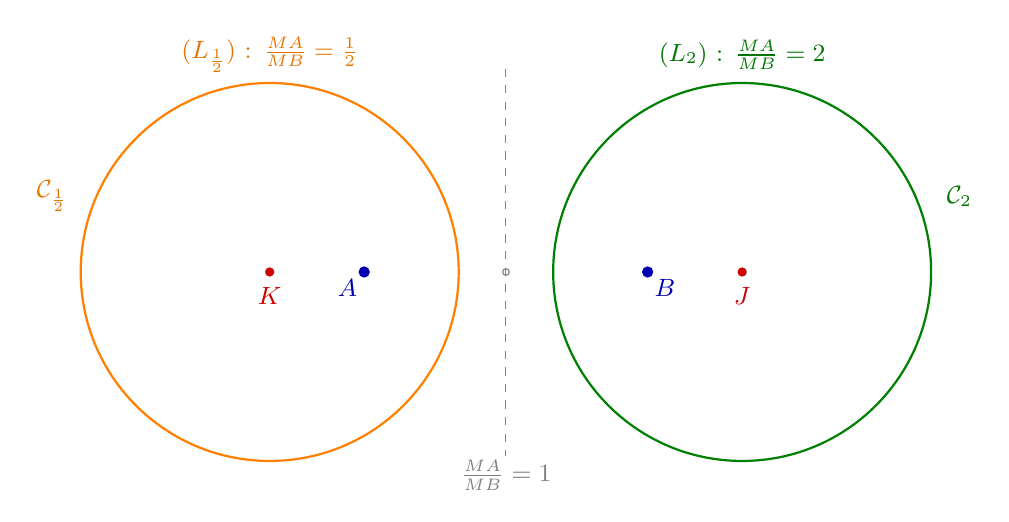
\begin{tikzpicture}[scale=0.60,>=latex]
  \draw[dashed,gray] (3,-4.3) -- (3,4.3);
  \draw[thick,green!50!black] (8,0) circle (4);
  \draw[thick,orange] (-2,0) circle (4);
  \fill[blue!70!black] (0,0) circle (3.4pt) node[below left=-1pt,font=\small] {$A$};
  \fill[blue!70!black] (6,0) circle (3.4pt) node[below right=-1pt,font=\small] {$B$};
  \fill[red!80!black] (8,0) circle (2.8pt) node[below=2pt,font=\small] {$J$};
  \fill[red!80!black] (-2,0) circle (2.8pt) node[below=2pt,font=\small] {$K$};
  \node[green!45!black,font=\small] at (8,4.6) {$(L_2)$ : $\frac{MA}{MB}=2$};
  \node[orange!90!black,font=\small] at (-2,4.6) {$(L_{\frac{1}{2}})$ : $\frac{MA}{MB}=\frac{1}{2}$};
  \node[gray,font=\small,fill=white,inner sep=1.5pt] at (3,-4.3) {$\frac{MA}{MB}=1$};
  \draw[gray,thin] (3,0) circle (2.0pt);
  \node[green!45!black,font=\small] at (12.6,1.6) {$\mathcal{C}_2$};
  \node[orange!90!black,font=\small] at (-6.6,1.6) {$\mathcal{C}_{\frac{1}{2}}$};
\end{tikzpicture}
